%-----------------------------------------------------------------------------------------------------------------------------------------------%
%	The MIT License (MIT)
%
%	Copyright (c) 2021 Jitin Nair
%
%	Permission is hereby granted, free of charge, to any person obtaining a copy
%	of this software and associated documentation files (the "Software"), to deal
%	in the Software without restriction, including without limitation the rights
%	to use, copy, modify, merge, publish, distribute, sublicense, and/or sell
%	copies of the Software, and to permit persons to whom the Software is
%	furnished to do so, subject to the following conditions:
%	
%	THE SOFTWARE IS PROVIDED "AS IS", WITHOUT WARRANTY OF ANY KIND, EXPRESS OR
%	IMPLIED, INCLUDING BUT NOT LIMITED TO THE WARRANTIES OF MERCHANTABILITY,
%	FITNESS FOR A PARTICULAR PURPOSE AND NONINFRINGEMENT. IN NO EVENT SHALL THE
%	AUTHORS OR COPYRIGHT HOLDERS BE LIABLE FOR ANY CLAIM, DAMAGES OR OTHER
%	LIABILITY, WHETHER IN AN ACTION OF CONTRACT, TORT OR OTHERWISE, ARISING FROM,
%	OUT OF OR IN CONNECTION WITH THE SOFTWARE OR THE USE OR OTHER DEALINGS IN
%	THE SOFTWARE.
%	
%
%-----------------------------------------------------------------------------------------------------------------------------------------------%

%----------------------------------------------------------------------------------------
%	DOCUMENT DEFINITION
%----------------------------------------------------------------------------------------

% article class because we want to fully customize the page and not use a cv template
\documentclass[a4paper,12pt]{article}

%----------------------------------------------------------------------------------------
%	FONT
%----------------------------------------------------------------------------------------

% % fontspec allows you to use TTF/OTF fonts directly
% \usepackage{fontspec}
% \defaultfontfeatures{Ligatures=TeX}

% % modified for ShareLaTeX use
% \setmainfont[
% SmallCapsFont = Fontin-SmallCaps.otf,
% BoldFont = Fontin-Bold.otf,
% ItalicFont = Fontin-Italic.otf
% ]
% {Fontin.otf}

%----------------------------------------------------------------------------------------
%	PACKAGES
%----------------------------------------------------------------------------------------
\usepackage{url}
\usepackage{parskip} 	

%other packages for formatting
\RequirePackage{color}
\RequirePackage{graphicx}
\usepackage[usenames,dvipsnames]{xcolor}
\usepackage[scale=0.9]{geometry}

%tabularx environment
\usepackage{tabularx}

%for lists within experience section
\usepackage{enumitem}

% centered version of 'X' col. type
\newcolumntype{C}{>{\centering\arraybackslash}X} 

%to prevent spillover of tabular into next pages
\usepackage{supertabular}
\usepackage{tabularx}
\newlength{\fullcollw}
\setlength{\fullcollw}{0.47\textwidth}

%custom \section
\usepackage{titlesec}				
\usepackage{multicol}
\usepackage{multirow}

%CV Sections inspired by: 
%http://stefano.italians.nl/archives/26
\titleformat{\section}{\Large\scshape\raggedright}{}{0em}{}[\titlerule]
\titlespacing{\section}{0pt}{10pt}{10pt}

%for publications
\usepackage[style=authoryear,sorting=ynt, maxbibnames=2]{biblatex}

%Setup hyperref package, and colours for links
\usepackage[unicode, draft=false]{hyperref}
\definecolor{linkcolour}{rgb}{0,0.2,0.6}
\hypersetup{colorlinks,breaklinks,urlcolor=linkcolour,linkcolor=linkcolour}
\addbibresource{citations.bib}
\setlength\bibitemsep{1em}

%for social icons
\usepackage{fontawesome5}

%debug page outer frames
%\usepackage{showframe}


% job listing environments
\newenvironment{jobshort}[2]
    {
    \begin{tabularx}{\linewidth}{@{}l X r@{}}
    \textbf{#1} & \hfill &  #2 \\[3.75pt]
    \end{tabularx}
    }
    {
    }

\newenvironment{joblong}[2]
    {
    \begin{tabularx}{\linewidth}{@{}l X r@{}}
    \textbf{#1} & \hfill &  #2 \\[3.75pt]
    \end{tabularx}
    \begin{minipage}[t]{\linewidth}
    \begin{itemize}[nosep,after=\strut, leftmargin=1em, itemsep=3pt,label=--]
    }
    {
    \end{itemize}
    \end{minipage}    
    }



%----------------------------------------------------------------------------------------
%	BEGIN DOCUMENT
%----------------------------------------------------------------------------------------
\begin{document}

% non-numbered pages
\pagestyle{empty} 

%----------------------------------------------------------------------------------------
%	TITLE
%----------------------------------------------------------------------------------------

% \begin{tabularx}{\linewidth}{ @{}X X@{} }
% \huge{Your Name}\vspace{2pt} & \hfill \emoji{incoming-envelope} email@email.com \\
% \raisebox{-0.05\height}\faGithub\ username \ | \
% \raisebox{-0.00\height}\faLinkedin\ username \ | \ \raisebox{-0.05\height}\faGlobe \ mysite.com  & \hfill \emoji{calling} number
% \end{tabularx}

\begin{tabularx}{\linewidth}{@{} X r @{}}
    \begin{minipage}[b]{\fullcollw}
        \Huge\textbf{Lin Mohan} \\[7.5pt]
        \small
        \href{https://github.com/linmoh}{\raisebox{-0.05\height}\faGithub\ linmoh} \ $|$ \ 
        \href{https://linmohan.net}{\raisebox{-0.05\height}\faGlobe \ linmohan.net} \\
        \href{https://linmohan.fun}{\raisebox{-0.05\height}\faBlog \ linmohan.fun} \ $|$ \ 
        \href{mailto:linmhwork@outlook.com}{\raisebox{-0.05\height}\faEnvelope \ linmhwork@outlook.com}
    \end{minipage} & 
    \begin{minipage}[b]{3cm} % 调整头像宽度
        \flushright
        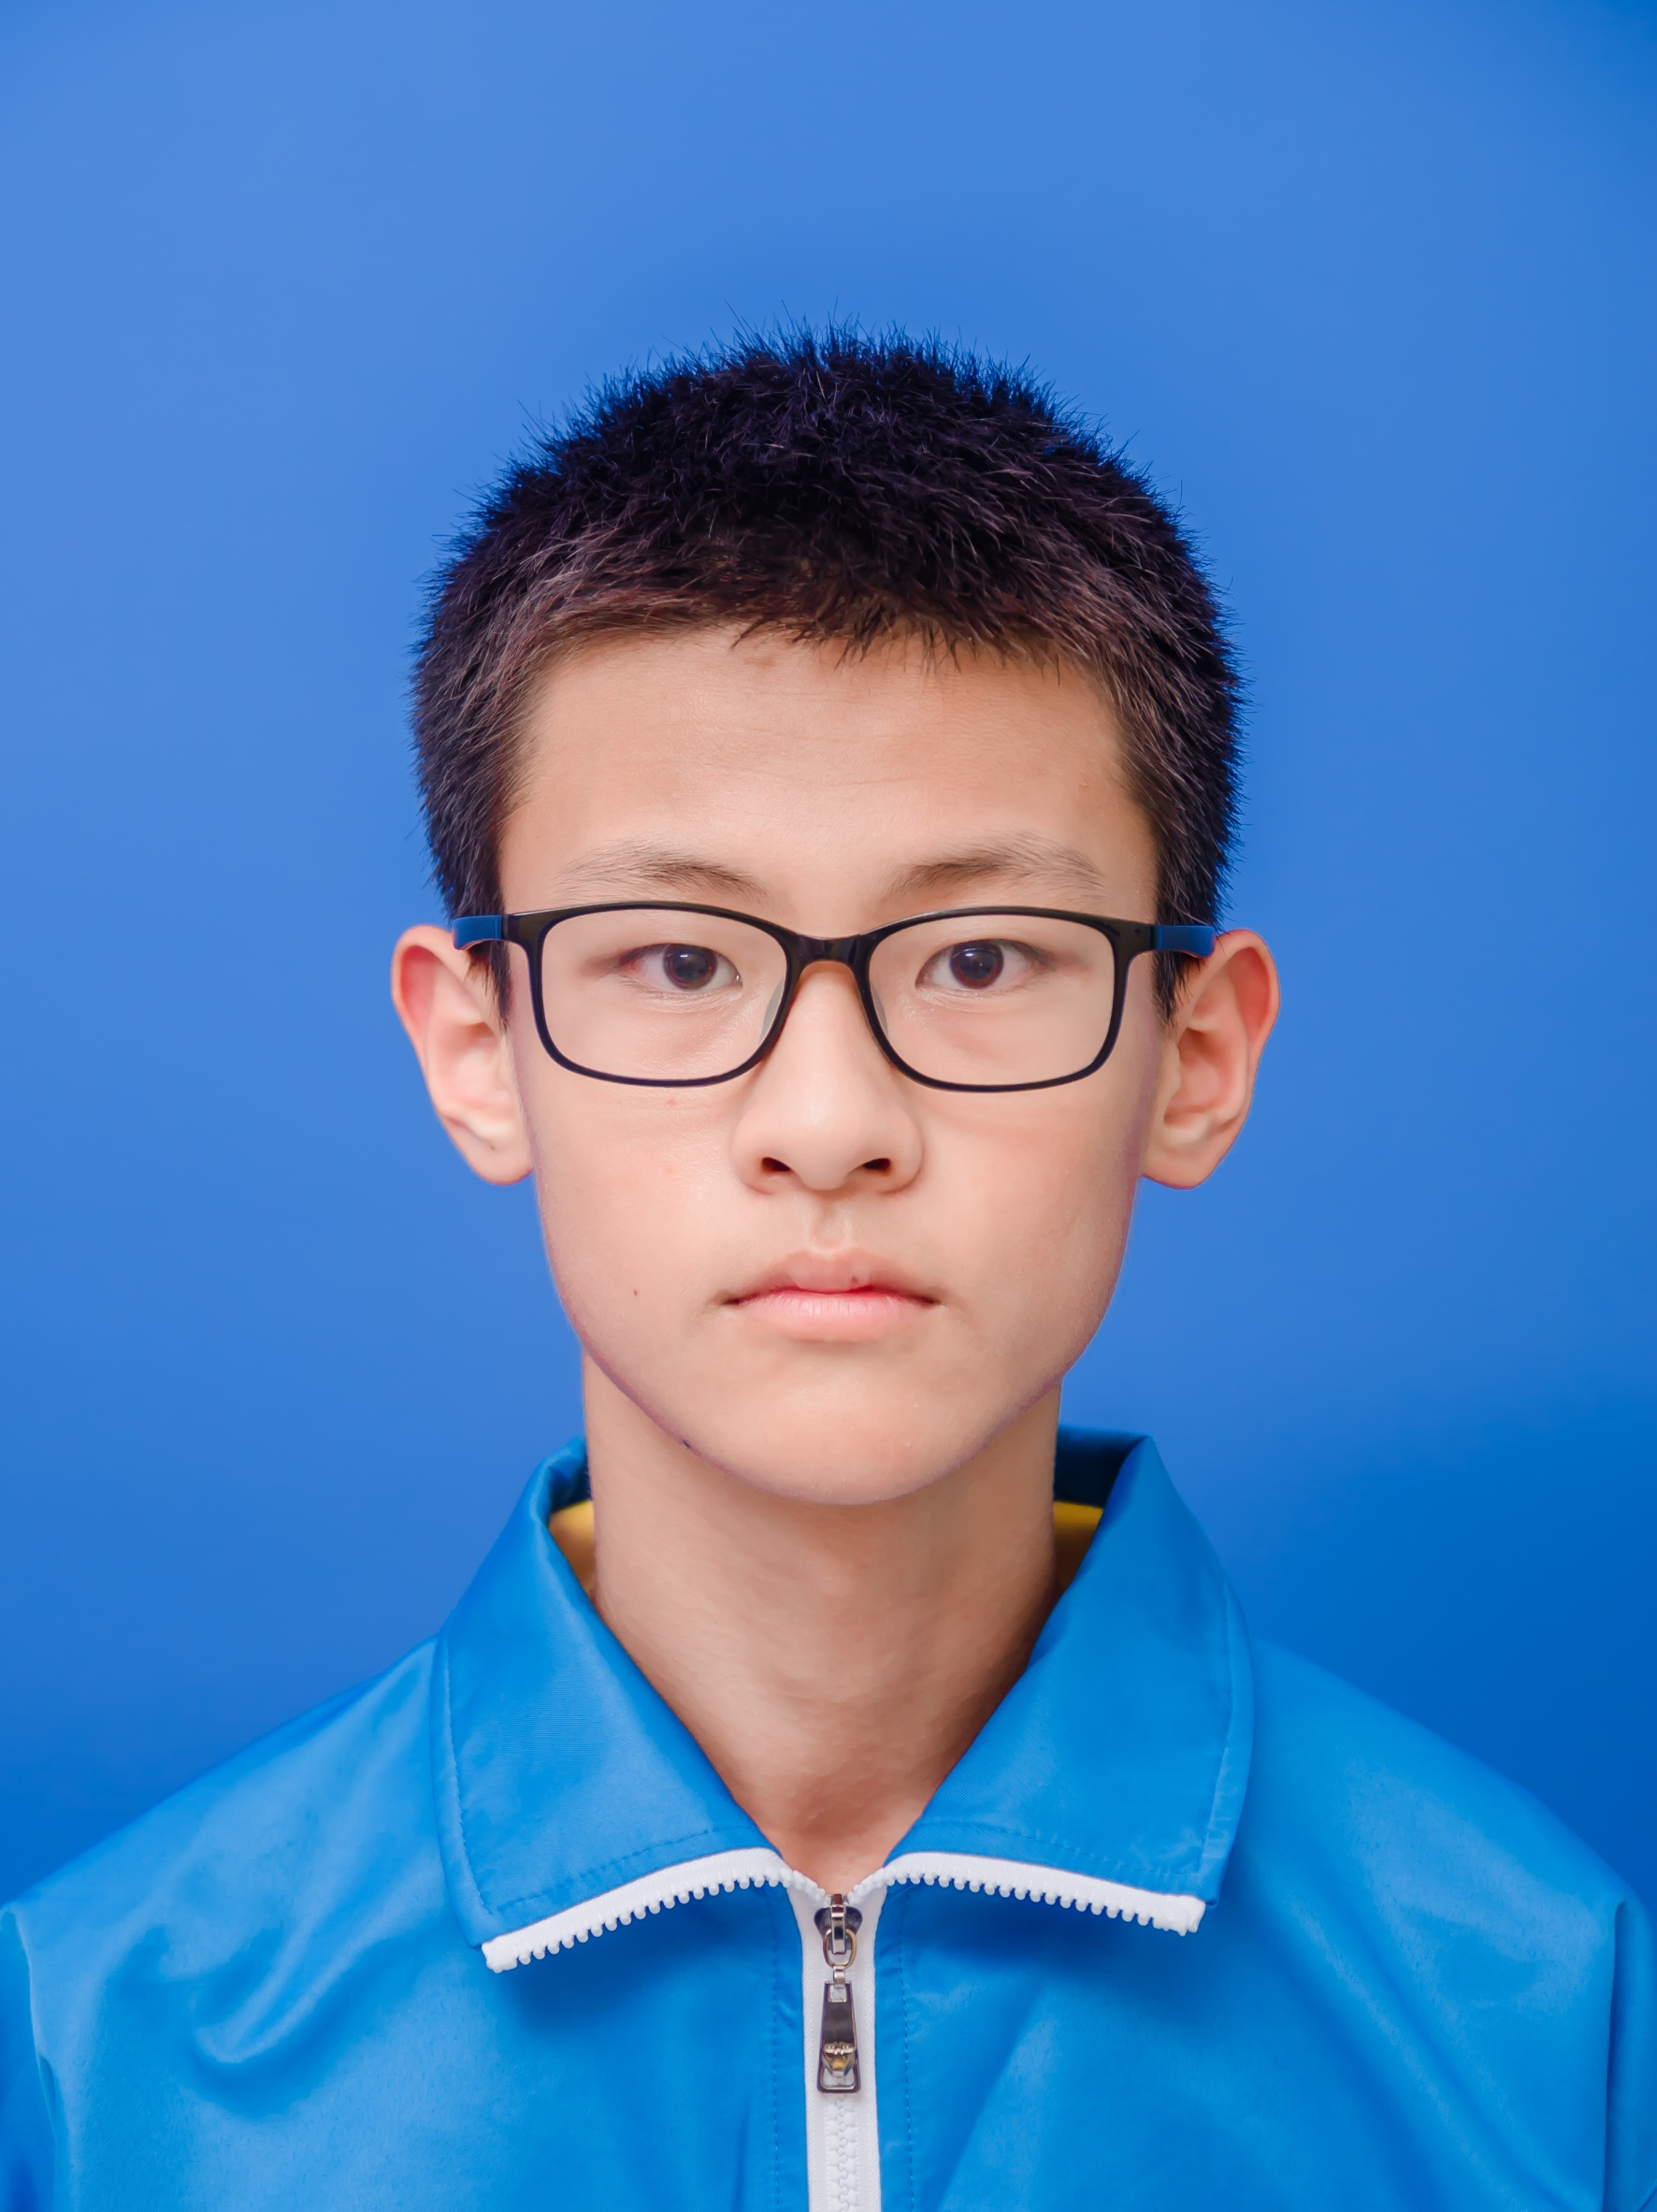
\includegraphics[width=2.8cm, height=2.8cm, keepaspectratio]{avatar.jpg}
    \end{minipage}
\end{tabularx}

%----------------------------------------------------------------------------------------
%   SUMMARY
%----------------------------------------------------------------------------------------
\section{Summary}
Grade 9 student and open-source enthusiast focused on \textbf{Systems Programming and Linux Kernels}; a \textbf{Linux Kernel contributor} with hands-on experience in PCI-related debugging and hardware-level analysis. As the founder of \textbf{TATEN}, a collaborative student developer community, I lead technical initiatives across age groups. Recognized for \textbf{Academic Excellence}, I was awarded \textbf{Direct Admission} to senior high school (skipping the Zhongkao) based on a consistent Top 40 ranking and all-around performance.

%----------------------------------------------------------------------------------------
% EXPERIENCE
%----------------------------------------------------------------------------------------
\section{Experience}

\begin{joblong}{Linux Kernel Bug Contributor}{Feb 2026}
\item \textbf{Issue Identification}: Identified and reported a PCI-related regression in the Linux kernel community.
\item \textbf{Debugging}: Investigated kernel driver behavior via system logs; verified system configurations and collaborated with upstream maintainers for resolution.
\item \textbf{Systems Knowledge}: Demonstrated deep understanding of low-level hardware-software interaction and kernel development workflows.
\end{joblong}

\begin{joblong}{Founder \& Lead Organizer, TATEN Community}{Jul 2025 - Present}
\item \textbf{Community Leadership}: Founded a technical community of 14+ members (ranging from middle school to undergraduates) to foster collaborative learning in CS.
\item \textbf{Project Management}: Spearheaded the development of \textbf{TATEN OJ} and \textbf{AniDay}, coordinating version control and technical roadmaps.
\item \textbf{Infrastructure}: Built and maintain the official portal (\href{https://taten.org}{taten.org}) and managed internal DevOps for community projects.
\end{joblong}
  
%----------------------------------------------------------------------------------------
% PROJECTS
%----------------------------------------------------------------------------------------
\section{Projects}

\begin{tabularx}{\linewidth}{ @{}l r@{} }
\textbf{AniDay} \small{(HTML, CSS, JavaScript)} & \hfill \href{https://aniday.xyz}{aniday.xyz} \\[3.75pt]
\multicolumn{2}{@{}X@{}}{A high-performance web application for querying anime character data. Optimized data retrieval logic and frontend responsiveness for a seamless user experience.}  \\
\end{tabularx}

\vspace{4pt}

\begin{tabularx}{\linewidth}{ @{}l r@{} }
\textbf{TATEN Online Judge} \small{(Vue, Rust)} & \hfill In Development \\[3.75pt]
\multicolumn{2}{@{}X@{}}{Designing a lightweight, containerized online judge system. Focus on secure code execution (sandboxing) and low-latency performance.}  \\
\end{tabularx}

\vspace{4pt}

\begin{tabularx}{\linewidth}{ @{}l r@{} }
\textbf{Student Computer Handbook} \small{(Markdown)} & \hfill In Progress \\[3.75pt]
\multicolumn{2}{@{}X@{}}{Authoring a comprehensive guide on modern computing for students, covering Linux basics, Git, and programming fundamentals.}  \\
\end{tabularx}

%----------------------------------------------------------------------------------------
%   HONORS & AWARDS
%----------------------------------------------------------------------------------------
\section{Honors \& Awards}

\begin{tabularx}{\linewidth}{@{}l X r@{}}
2025 & \textbf{First Prize}, 26th Jinan Student Information Literacy Activity & Municipal \\
     & \textit{Project: Algorithm and Data Visualization Toolset} & \\
2024 & \textbf{Second Prize}, 25th Jinan Student Information Literacy Activity & Municipal \\
     & \textit{Project: Educational Game Collection} & \\
2023 & \textbf{Municipal Outstanding Student}, Jinan Education Bureau & City-level \\
     & \textit{Selected from the top 0.9\% of students for exemplary academic performance, moral character, and all-around comprehensive qualities.} & \\
2023 & \textbf{Second Prize}, 24th Jinan Student Information Literacy Activity & Municipal \\
     & \textit{Project: Conway's Game of Life (Simulation)} & \\
\end{tabularx}

%----------------------------------------------------------------------------------------
%   EDUCATION
%----------------------------------------------------------------------------------------
\section{Education}

\begin{tabularx}{\linewidth}{@{}l X@{}}
2025 -- 2029 & \textbf{Pingyin Experimental Senior High School}, Jinan, China \\
2023 -- 2025 & \textbf{Pingyin Experimental Senior High School (Junior Division)} \\
\end{tabularx}

%----------------------------------------------------------------------------------------
%   SKILLS
%----------------------------------------------------------------------------------------
\section{Skills}

\begin{tabularx}{\linewidth}{@{}l X@{}}
\textbf{Systems \& Low-level} & \normalsize{Linux (Arch Linux), Kernel Debugging, Shell Scripting, Git, DevOps} \\
\textbf{Programming} & \normalsize{C/C++, Python, Rust, Data Structures \& Algorithms, JavaScript} \\
\textbf{Web Development} & \normalsize{Vue.js, HTML5/CSS3, Frontend Performance Optimization} \\
\textbf{Multimedia Tools} & \normalsize{Blender (3D Modeling), AE/PR (Video Synthesis), PS/AI (Visual Design)} \\
\end{tabularx}

\vfill
\center{\footnotesize Last updated: \today}

\end{document}
